\documentclass{article}
\usepackage{ifxetex}
\ifxetex
  \usepackage{fontspec}
\else
  \usepackage[T1]{fontenc}
  \usepackage[utf8]{inputenc}
  \usepackage{lmodern}
\fi
\title{Problem Set 8}
\author{%
    Ishan Pranav
\\  MATH-UA 120 Discrete Mathematics
}
\date{due December 8, 2023}
\usepackage[headings=runin-fixed-nr]{exsheets}
\makeatletter
    \newcommand{\stepenumdepth}{\advance\@enumdepth\@ne}
\makeatother
\SetupExSheets{
    question/pre-body-hook=\stepenumdepth,
    solution/pre-body-hook=\stepenumdepth,
}
\DeclareInstance{exsheets-heading}{runin-nn-np}{default}{
    runin = true,
    title-post-code = .\space,
    join = {
        main[r,vc]title[l,vc](0pt,0pt);
    }
}
\newif\ifshowsolutions
\showsolutionstrue
\ifshowsolutions
    \SetupExSheets{
        question/pre-hook=\itshape,
        solution/headings=runin-nn-np,
        solution/print=true,
        solution/name=Answer
    }%
    \makeatletter%
    \pretocmd{\@title}{Answers to }%
    \makeatother%
\else
    \SetupExSheets{solution/print=false}
\fi

% Bug workaround: http://tex.stackexchange.com/a/146536/1402
%\newenvironment{exercise}{}{}
\RenewQuSolPair{question}{solution}
%\let\answer\solution
%\let\endanswer\endsolution
\usepackage{manfnt}
\newcommand{\danger}{\marginpar[\hfill\dbend]{\dbend\hfill}}
\newcommand{\Z}{\mathbb{Z}}
\newcommand{\N}{\mathbb{N}}
\newcommand{\modulo}{\text{ mod }}
\newcommand{\divisor}{\text{ div }}
\usepackage{tikz}
\tikzstyle{vertex}=[circle,draw,fill=none,inner sep=0pt,outer sep=0pt, minimum width=1ex]
\tikzstyle{edge}=[draw,thick]
\usepackage{multirow, multicol}
\usepackage{amsmath, amsthm, amssymb}
\usepackage{amsfonts}
\usepackage{siunitx}
\DeclareSIUnit\pound{lb}
\DeclareMathOperator{\dom}{dom}
\DeclareMathOperator{\im}{im}
\DeclareMathOperator{\sgn}{sgn}
\usepackage{hyperref}
\newtheorem*{theorem}{Theorem}
\theoremstyle{definition}
\newtheorem*{definition}{Definition}
\newenvironment{note}{\noindent\emph{Note}.}{}
\begin{document}
\maketitle
These are to be written up and turned in to Gradescope.\\

\ifshowsolutions
    \SetupExSheets{solution/print=true}
\else
    \danger
 \underline{ \LaTeX  Instructions:}  You can view the source (\texttt{.tex}) file to get some more examples of \LaTeX{} code.  I have commented the source file in places where new \LaTeX{} constructions are used.
  
  Remember to change \verb|\showsolutionsfalse| to \verb|\showsolutionstrue|
    in the document's preamble 
    (between \verb|\documentclass{article}| and \verb|\begin{document}|)
\fi
\section*{Assigned Problems}
\begin{question}
    \begin{enumerate}
        \item Find $d = \gcd(29341,1739)$, and integers $x$ and $y$ such that $29341x + 1739y = d$.
        \item Prove that 7 cannot be expressed as an integral linear combination of 29341 and 1739.
    \end{enumerate}
\end{question}
\begin{solution}
\begin{enumerate}
\item Let $d=\gcd(29341,1739)$. Observe
\begin{align*}
d
&=\gcd(29341,1739)\\
&=\gcd(1739,29341 \modulo 1739)&\text{(note }29341-16\cdot 1739=1517\text{)}\\
&=\gcd(1517,1739 \modulo 1517)&\text{(note }1739-1\cdot 1517=222\text{)}\\
&=\gcd(222,1739 \modulo 222)&\text{(note }1517-6\cdot 222=185\text{)}\\
&=\gcd(185,222 \modulo 185)&\text{(note }222-1\cdot 185=37\text{)}\\
&=\gcd(37,185 \modulo 37)&\text{(note }185-5\cdot 37=0\text{)}\\
&=37.
\end{align*}
Consider $37=29341x+1739y$. Observe
\begin{align*}
0\cdot 29341+1\cdot 1739&=1739\\
1\cdot 29341-16\cdot 1739&=1517\\
-1\cdot 29341+17\cdot 1739&=222\\
7\cdot 29341-118\cdot 1739&=185\\
29341x+1739y&=37.
\end{align*}
Thus $x=-8$ and $y=135$ is a possible solution.
\item\textit{Claim. } 7 cannot be expressed as an integral linear combination of 29341 and 1739.
\begin{proof}
Assume, for the sake of contradiction, that 7 can be expressed as an integral linear combination of 29341 and 1739. Note $\gcd(29341,1739)=37$ is the smallest positive integer expressible as a linear combination of $29341\in\Z$ and $1739\in\Z$. However, $7\in\Z$ and $0<7<37$, which is a contradiction. Ergo our assumption is false: 7 is not expressible as a linear combination of 29341 and 1739. 
\end{proof}
\end{enumerate}
\end{solution}
\begin{question}
    \begin{enumerate}
        \item Disprove: There exist integers $a$ and $b$ such that $a+b=100$ and $\gcd(a, b)=8$.
        \item Prove: There exist infinitely many pairs of integers $(a,b)$ such that $a+b=87$ and $\gcd(a, b)=3$.
    \end{enumerate}
\end{question}
\begin{solution}
\begin{enumerate}
\item\small{LEMMA.}

\textit{Claim. }There do not exist $a\in\Z$ and $b\in\Z$ where $a+b=100$ and $\gcd(a,b)=8$.
\begin{proof}
Assume, for the sake of contradiction, there exist $a\in\Z$ and $b\in\Z$ where $a+b=100$ and $\gcd(a,b)=8$. Since $\gcd(a,b)=8$, we know $8\mid a$ and $8\mid b$. Thus there exist $k_1\in\Z$ and $k_2\in\Z$ where $a=8k_1$ and $b=8k_2$. Observe
\begin{align*}
a+b
&=8k_1+8k_2\\
&=8(k_1+k_2)\\
&=100.
\end{align*}
There exists $(k_1+k_2)\in\Z$ where $100=8(k_1+k_2)$. Thus $8\mid(a+b)$. However, $a+b=100$ and, of course, $8\nmid 100$. This is a contradiction. Thus our assumption is false: There do not exist $a\in\Z$ and $b\in\Z$ where $a+b=100$.
\end{proof}
\small{PROPOSITION.}

\textit{Claim. }Disprove: There exist integers $a$ and $b$ such that $a+b=100$ and $\gcd(a,b)=8$.
\begin{proof}
The claim is false by lemma.
\end{proof}
\item\textit{Claim. }There exist infinitely many pairs of integers $(a,b)$ such that $a+b=87$ and $\gcd(a, b)=3$.
\begin{proof}
Let $X=\{x\in\Z:29\nmid x\}$.

Let $Y=\{(a,b)\in\Z^2:a+b=87~\text{ and}~\gcd(a,b)=3\}$.

Let $f$ be the relation $\{(x,(3x,87-3x)):x\in X\}$.

(Function) Let $(x_0,y_1),(x_0,y_2)\in f$. Then $y_1=(3x_0,87-3x_0)$ and $y_2=(3x_0,87-3x_0)$. Thus $y_1=y_2$. Therefore $f$ is a function.

(Domain) Note $\dom{f}=X$ by construction.

(Image) Let $(x,(a,b))\in f$. Note also $a\in\Z$ and $b\in\Z$ so $(a,b)\in\Z^2$. Note
\[(a+b)=(3x+(87-3x))=87.\]
Note also
\[\gcd(a,b)=\gcd(3x,87-3x)=\gcd(3x,3(29-x)).\]

Since $x\in X$, we have $x\in\Z$. Since $a=3x$, we have $3\mid a$. Since there exists $(29-x)\in\Z$ where \[b=(87-3x)=3(29-x)\] we have $3\mid b$. Therefore, 3 is a common divisor of $a$ and $b$. 

Since every integer can be expressed as a product of integer divisors, and because every pair of integers has a common divisor, there exist $k_1,k_2,k_3\in\Z$ where $x=k_1k_2$ and $(29-x)=k_1k_3$. Note
\[(x-(29-x))=(k_1k_2-k_1k_3)=k_1(k_2-k_3).\]
So $k_1\mid(x-(29-x))$. Since $(x-(29-x))=(2x-29)$, we have $k_1\mid(2x-29)$. Note $k_1\mid x$, so $k_1\mid 2x$. So it must be that $k_1\mid 29$. However, since 29 is prime, $k_1=1$ or $k_1=29$. But since $x\in X$, we have $29\nmid x$. Thus $k_1\neq 29$. Therefore $k_1=1$. The only common divisor between $x$ and $(29-x)$ is 1. Thus $\gcd(x,29-x)=1$. Since $a=3x$ and $b=3(29-x)$, the common divisors of $a$ and $b$ are 1 and 3. Since $1<3$, we have $\gcd(a,b)=3$. 

Since, $(a,b)\in\Z^2$ with $a+b=87$ and $\gcd(a,b)=3$, we have $(a,b)\in Y$. Therefore $\im{f}\subseteq Y$.

(Injective) Let $x_1,x_2\in X$. Suppose $f(x_1)=f(x_2)$. Then $(3x_1,87-3x_1)=(3x_2,87-3x_2)$. Since $3x_1=3x_2$, we have $x_1=x_2$. Therefore $f$ is injective.

(Surjective) Let $(a',b')\in Y$. Note $3\mid a'$. We can construct $x'=\frac{a'}{3}\in\Z$ where $f(x')=(a',b')$. So $\im{f}=Y$. Therefore $f$ is surjective.

Hence, $f:X\to Y$ is bijective. Note $X$ is an infinite set. Since $f$ is bijective, $Y$ is an infinite set. Ergo there are infinitely many pairs of integers $(a,b)$ where $a+b=87$ and $\gcd(a,b)=3$.
\end{proof}
\end{enumerate}
\end{solution}
\begin{question}
    \begin{enumerate}
        \item Let $a, b, c\in \Z$ such that $a$ and $b$ are relatively prime. Prove that if $a\mid c$ and $b\mid c$, then $(ab)\mid c$.
        \item Explain why part (a) is false if $a$ and $b$ are not relatively prime.
    \end{enumerate}
\end{question}
\begin{solution}
\begin{enumerate}
\item\textit{Claim. }Let $a,b,c\in\Z$ where $a$ and $b$ are relatively prime. If $a\mid c$ and $b\mid c$, then $ab\mid c$.
\begin{proof}
Let $a,b,c\in\Z$ where $a$ and $b$ are relatively prime. Suppose $a\mid c$ and $b\mid c$. Since $a$ and $b$ are relatively prime, $\gcd(a,b)=1$. Since $\gcd(a,b)=1$ is the smallest positive integer of which $a$ and $b$ can be expressed as an integer linear combination, there exist $x,y\in\Z$ where $ax+by=1$. Since $a\mid c$, there exists $k_1\in\Z$ where $c=ak_1$. Since $b\mid c$, there exists $k_2\in\Z$ where $c=bk_2$. Observe
\begin{align*}
ax+by&=1\\
c(ax+by)&=c\\
cax+cby&=c\\
bk_2ax+ak_1by&=c\\
ab(k_2x+k_1y)&=c.
\end{align*}
There exists $(k_2x+k_1y)\in\Z$ where $c=(k_2x+k_1y)ab$. Hence, $ab\mid c$.
\end{proof}
\item Let $a,b,c\in\Z$ where $a\mid c$ and $b\mid c$ where $a$ and $b$ are not relatively prime. If $a$ and $b$ are not relatively prime, then there exist cases where $ab>c$, and thus, $ab\nmid c$. We know $c$ can be expressed as a product of $n$ prime factors where $q_i$ represents a unique prime factor and $a_i$ represents its count for $i\in\N$ where $i\leq n$:
\[c=\prod_{i=1}^n{q_i^{a_i}}.\]
If $a$ and $b$ are not relatively prime then, letting $d=\gcd(a,b)$, we have $d>1$. This means that $a$ and $b$ share at least one prime factor. There exists $q^*\in\Z$ where $q^*\mid a$ and $q^*\mid b$ and $q^*$ is prime.

Now there exist $k_1,k_2\in\Z$ where $a=k_1q^*$ and $b=k_2q^*$. Since $a\mid c$, we have $k_1q^*\mid c$. Since $b\mid c$, we have $k_2q^*\mid c$. Thus $k_1k_2q^*\mid c$. However, we have no guarantee that $k_1k_2(q^*)^2\mid c$. That is, we do not know if there is more than one instance of  $q^*$ in the prime factorization of $c$. Thus we cannot be certain that $ab\mid c$.

Using this technique, we can construct a counterexample. Consider $4,6,12\in\Z$. Note $4\mid 12$ and $6\mid 12$. Note also $\gcd(4,6)=2$, so $4$ and $6$ are not relatively prime. However, $4\cdot 6=24$ and of course $24\nmid 12$. Hence disproven.
\end{enumerate}
\end{solution}
\begin{question} 
 Consider the following graph $G$.
     \begin{center}
    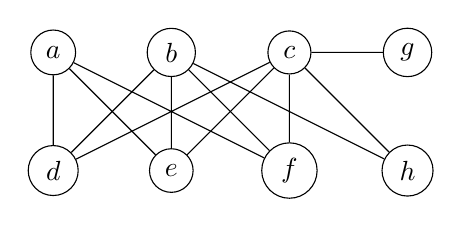
\begin{tikzpicture}[
        every node/.append style={draw,circle}
    ]
        \node (A) at (-1.5, 0) {$a$};
        \node (B) at (0, 0)    {$b$};
        \node (C) at (1.5, 0)  {$c$};
        \node (D) at (-1.5, -1.5) {$d$};
        \node (E) at (0, -1.5)   {$e$};
        \node (F) at (1.5, -1.5) {$f$};
        \node (G) at (3, 0)   {$g$};
        \node (H) at (3, -1.5) {$h$};
        \draw (A) -- (D) -- (C) -- (F) -- (A);
        \draw (A) -- (E) -- (C);
        \draw (D) -- (B) -- (F);
        \draw (G) -- (C) -- (H) -- (B) -- (E);
    \end{tikzpicture}
    \end{center}
    
\begin{enumerate}
	\item Write out the ordered pair $G=(V, E)$.
	\item What is the order of $G$?
	\item What is the size of $G$?
	\item What is $N(b)$?
	\item What is $d_G(c)$?
	\item What is $\Delta(G)$?
	\item What is $\delta(G)$?
	\item What elements are the vertex $a$ adjacent to?
	\item What elements are the vertex $f$ incident with?
	\item Is $G$ regular? Briefly explain why or why not.
	\end{enumerate}
\end{question}
\begin{solution}
\begin{enumerate}
\item\begin{align*}
G=(V,E)=(\{a,b,c,d,e,f,g,h\},\{\\
\{a,d\},\{a,e\},\{a,f\},\\
\{b,d\},\{b,e\},\{b,f\},\{b,h\},\\
\{c,d\},\{c,e\},\{c,f\},\{c,h\},\{c,g\}\}).
\end{align*} An undirected graph is an ordered pair where the first element is the set of vertices and the second element is the set of edges, where each edge is two-element set of vertices.
\item The order of $G$ is the number of vertices in $G$. Thus the order of $G$ is $|V|=8$.
\item The size of $G$ is the number of edges in $G$. Thus the order of $G$ is $|E|=12$.
\item The neighborhood of $b$, $N(b)$, represents the set of vertices adjacent to vertex $b$. Thus $N(b)=\{d,e,f,h\}$.
\item $d_G(c)$ represents the degree of vertex $c$ in $G$. Thus $d_G(c)=|N(c)|=5$.
\item $\Delta(G)$ represents the maximum degree of $G$. Thus $\Delta(G)=d_G(c)=5$.
\item $\delta(G)$ represents the minimum degree of $G$. Thus $\delta(G)=d_G(g)=1$.
\item Vertex $a$ is adjacent to vertices $d$, $e$, and $f$ because for graph $G=(V,E)$, we have $a,d,e,f\in V$ and $\{a,d\},\{a,e\},\{a,f\}\in E$.
\item Vertex $f$ is incident with edges $\{a,f\}$, $\{b,f\}$, and $\{c,f\}$ because for graph $G=(V,E)$, we have $f\in V$ and $\{a,f\},\{b,f\},\{c,f\}\in E$.
\item No, $G$ is not regular. In a regular graph $(V',E')$, there exists a number $k$ where for all vertices $v\in V'$, we have $d_{(V',E')}(v)=k$. Consider $b,c\in G$. Note $d_G(c)=5$ and $d_G(g)=1$. However, $5\neq 1$. Thus $G$ is not regular.

Put another way, in a regular graph $(V,E)$, we have $\Delta((V,E))=\delta((V,E))$. However $(\Delta(G)=5)\neq(\delta(G)=1)$. Thus $G$ is not regular.
\end{enumerate}
\end{solution}
\begin{question}
     Let $G=(V,E)$ be a graph. Prove by induction: 
\begin{quote}
The sum of the degrees of the vertices in $G$ is twice the number of edges.
\end{quote}	
\end{question}
\begin{solution}
\textit{Claim. }Let $G=(V,E)$ be a graph. Then \[\sum_{v\in V}{d_G(v)}=2|E|.\]
\begin{proof}
Let $G=(V,E)$ be a graph. We will demonstrate $\sum_{v\in V}{d_G(v)}=2|E|$ by induction on $|E|$.
\begin{description}
\item[Basis case.] Consider a graph $G_0=(V_0,E_0)$ where $|E_0|=0$. Since there are no edges in $E_0$, for all $v_0\in V_0$, we have $d_{G_0}(v_0)=0$. Therefore \[\sum_{v_0\in V_0}{d_{G_0}(v_0)}=\sum_{v_0\in V_0}{0}=2(0).\]
\item[Inductive hypothesis.] Let $k\in\N$. Consider a graph $G_k=(V_k,E_k)$ where $|E_k|=k$. Assume that \[\sum_{v\in V_k}{d_{G_k}(v)}=2k.\]
\item[Induction step.] Consider a graph $G^*=(V^*,E^*)$ where $|E^*|=k+1$. Note $k+1>0$ so $|E^*|>0$. Thus $E^*\neq\emptyset$. By omitting an edge $e\in E^*$, we can construct a graph $G'=(V^*,E^*-\{e\})$. Of course \[|E^*-\{e\}|=((k+1)-1)=k.\] By the induction hypothesis, we have \[\sum_{v\in V^*}{d_{G'}(v)=2|E^*-\{e\}|=2k}.\] Recall that $e\in E^*$. There exist vertices $u,v\in V^*$ where $e=\{u,v\}$. Since $e$ is a set, $u\neq v$. Note that $d_{G^*}(u)=d_{G'}(u)+1$ because in graph $G^*$, vertex $u$ is connected to vertex $v$ by edge $e$. Symmetrically, $d_{G^*}(v)=d_{G'}(v)+1$. Let $W=V^*-\{u,v\}$. The inclusion or omission of $e$ has no effect on the degree of any other vertex $w\in W$. Thus
\begin{align*}
\sum_{v\in V^*}{d_{G^*}(v)}
&=\left(d_{G^{'}}(u)+1\right)+\left(d_{G^{'}}(v)+1\right)+\sum_{w\in W}{d_{G^{'}}(w)}\\
&=1+1+d_{G^{'}}(u)+d_{G^{'}}(v)+\sum_{w\in W}{d_{G^{'}}(w)}\\
&=1+1+\sum_{v\in V^*}{d_{G^{'}}(v)}\\
&=2+2k\\
&=2(k+1).
\end{align*}
This completes the inductive step.
\end{description}
Hence, by the principle of mathematical induction, for any graph $G=(V,E)$, we have
\[\sum_{v\in V}d_G(v)=2|E|.\]
\end{proof}
\end{solution}
\end{document}